\documentclass{acm_proc_article-sp}
%\documentclass{paper}
\usepackage{subfigure}
\begin{document}

\title{Shadow Computing}
\subtitle{An Energy-Aware Resiliency Scheme for Cloud Computing}
%
% You need the command \numberofauthors to handle the 'placement
% and alignment' of the authors beneath the title.
%
% For aesthetic reasons, we recommend 'three authors at a time'
% i.e. three 'name/affiliation blocks' be placed beneath the title.
%
% NOTE: You are NOT restricted in how many 'rows' of
% "name/affiliations" may appear. We just ask that you restrict
% the number of 'columns' to three.
%
% Because of the available 'opening page real-estate'
% we ask you to refrain from putting more than six authors
% (two rows with three columns) beneath the article title.
% More than six makes the first-page appear very cluttered indeed.
%
% Use the \alignauthor commands to handle the names
% and affiliations for an 'aesthetic maximum' of six authors.
% Add names, affiliations, addresses for
% the seventh etc. author(s) as the argument for the
% \additionalauthors command.
% These 'additional authors' will be output/set for you
% without further effort on your part as the last section in
% the body of your article BEFORE References or any Appendices.

\numberofauthors{1} %  in this sample file, there are a *total*
% of EIGHT authors. SIX appear on the 'first-page' (for formatting
% reasons) and the remaining two appear in the \additionalauthors section.
%
\author{
% You can go ahead and credit any number of authors here,
% e.g. one 'row of three' or two rows (consisting of one row of three
% and a second row of one, two or three).
%
% The command \alignauthor (no curly braces needed) should
% precede each author name, affiliation/snail-mail address and
% e-mail address. Additionally, tag each line of
% affiliation/address with \affaddr, and tag the
% e-mail address with \email.
%
% 1st. author
\alignauthor
Bryan Mills\raisebox{4pt}{$\ast$}, Taieb Znati\raisebox{4pt}{$\ast$$\dagger$}, Rami Melhem\raisebox{4pt}{$\ast$}\\
       \affaddr{Department of Computer Science\raisebox{4pt}{$\ast$}}\\
       \affaddr{Telecommunications Program\raisebox{4pt}{$\dagger$}}\\
       \affaddr{University of Pittsburgh}\\
       \affaddr{Pittsburgh, PA  15260}\\
       \email{(bmills, znati, melhem)@cs.pitt.edu}
}

\maketitle
\thispagestyle{empty}

%%\begin{IEEEkeywords}
%%shadow computing, fault tolerance, scheduling, resiliency
%%\end{IEEEkeywords}

\begin{abstract}
With the concerted efforts from researchers in hardware, software, algorithm, and data management, HPC is moving towards extreme-scale, featuring a computing capability of quintillion ($10^{18}$) FLOPS. 
As we approach the new era of computing, however, several daunting scalability challenges remain to be conquered. Delivering extreme-scale performance will require a computing platform that supports billion-way parallelism, necessitating a dramatic increase in the number of computing, storage, and networking components. At such a large scale, failure would become a norm rather than an exception, driving the system to significantly lower efficiency with unprecedented amount of power consumption. %The frequency and diversity of failures,  as well as the challenge of power, call for rethinking of the fault tolerance problem. 

To tackle this challeng, we propose an adaptive and power-aware algorithm, referred to as Lazy Shadowing, as an efficient and scalable approach to achieve high-levels of resilience, through forward progress, in extreme-scale, failure-prone computing environments. 
Lazy Shadowing associates with each process a ``shadow" (process) that executes at a reduced rate, and opportunistically rolls forward each shadow to catch up with the its leading process during failure recovery.
%overlaps the recovery time after each failure with the time needed to roll forward the shadows to a consistent state.
Compared to existing fault tolerance methods, our approach can achieve 20\% energy saving with potential reduction in solution time at scale.

\end{abstract}

\section{Introduction}
\label{intro}
As our reliance on IT continues to increase, the complexity and urgency of the problems our society will face 
in the future drives us to build more powerful and accessible computer systems. Among the different types of 
computer systems, High Performance Computing (HPC) and Cloud Computing systems are the two most powerful ones. 
For both, the computing power attributes to the massive amount of parallelism, which is enabled by 
the massive amount of CPU cores, memory modules, communication devices, storage components, etc. 

Since CPU frequency flattened out in early 2000s, parallelism has become the ``golden rule" to boost performance. 
In HPC, Terascale performance was achieved in the late 90’s with fewer than 10,000 heavyweight single-core processors. 
A decade later, petascale performance required about ten times more processors with multiple cores on each processor. Nowadays, a race
is underway to build the world's first exascale machine to accelerate scientific discoveries and breakthroughs. It is 
projected that an exascale machine will achieve billion-way parallelism by using one million sockets each supporting 
1,000 cores~\cite{doe_ascr_exascale_2011,top_ten_2014}. 

Similar trend is happening in Cloud Computing. 
As the demand for Cloud Computing accelerates, cloud service providers  
will be faced with the need to expand their underlying infrastructure to ensure the expected levels of performance, reliability and cost-effectiveness. 
As a result, lots of large-scale data centers have been and are being built by IT companies
to exploit the power and economies of scale. 
For example, Google, Facebook, and Rackspace have hundreds of thousands 
of web servers in dedicated data centers to support their business. 

Unfortunately, several challenging issues come with the increase in system scale. As today's HPC and Cloud Computing systems grow to 
meet tomorrow's compute power demand, the behavior of the systems will be increasingly difficult to specify, predict and manage. 
This upward trend, in terms of scale and complexity, has a direct negative effect on the overall system reliability. 
%Even with the expected improvement in the reliability of future computing technology, the rate of system level failures will 
%dramatically increase with the number of components, possibly by several orders of magnitude. 
At the same time, the rapid 
growing power consumption, as a result of the increase in system components, is another major concern. 
%It is reported that 
%the power required to run the machines as well as cool them has become the largest cost factor in a large-scale system's operating 
%expenses.  
At future extreme-scale, failure would become a norm rather than an exception, 
driving the system to significantly lower efficiency with unprecedented amount of power consumption. 

\section{Problem Statement}

The system scale needed to address our future computing needs will come at the cost of increasing complexity, unpredictability, 
and operating expenses. As we approach future extreme-scale computing, two of the biggest challenges will be system resilience and power 
consumption, both being direct consequences of the dramatic increase in the number of system components~\cite{exa_challenge_2010,snir2014addressing}. 

Regardless of the reliability of individual component, the system level failure rate will continue to increase as the number of 
components increases, possibly by several orders of magnitude. It is projected that the Mean Time Between Failures (MTBF) of future extreme-scale systems will be at the order of hours or even minutes, meaning 
that many failures will occur every day~\cite{Bergman08exascalecomputing}. Without an efficient fault tolerance mechanism, faults will be so frequent that the applications running on the 
systems will be continuously interrupted, requiring the execution to be restarted every time there is a failure. 

Also thanks to the continuous growth in system components, there has been a steady rise in power consumption in large-scale distributed systems. 
In 2005, the peak power consumption of a single supercomputer reached 3.2 Megawatts. This number was doubled only after 5 years, and reached 17.8 
Megawatts with a machine of 3,120,000 cores in 2013. Recognizing this rapid upward trend, the U.S. Department of Energy has set 20 
megawatts as the power limit for future exascale systems, 
challenging the research community to provide a 1000x improvement in performance with only a 10x increase in power~\cite{exa_challenge_2010}. 
This huge imbalance makes system power a leading design constraint on the path to exascale. 

Today, two approaches exist for fault tolerance. The first approach is rollback recovery, which rolls back and restarts the execution 
every time there is a failure. This approach is often equipped with checkpointing to periodically save the execution state to a 
stable storage so that execution can be restarted from a recent checkpoint in the case of a failure~\cite{Elnozahy:02:Survey,kalaiselvi_sadhana_2000,Chandy:1985:DSD:214451.214456}. 
Although checkpointing is the most widely used technique in today's HPC systems, it may not scale to 
future extreme-scale systems~\cite{ferreira_sc_2011,elnozahy_dsc_2004,4367962}. Given the anticipated increase in system level failure rates and the time to checkpoint large-scale 
compute-intensive and data-intensive applications, the time required to periodically checkpoint an application 
and restart its execution will approach the system's MTBF~\cite{Cappello:2009:TER:1640402.1640428}. Consequently, applications will make little forward progress, thereby 
reducing considerably the overall system efficiency. 

The second approach, referred to as process replication, exploits hardware redundancy and executes multiple instances of the same task 
in parallel to overcome failure and guarantee that at least one task instance reaches completion~\cite{bartlett_1981_nonstop,tsai_isads_2011,ferreira_sc_2011}. Although this approach is extensively used 
to deal with failures in 
Cloud Computing and mission critical systems, it has 
never been used in any HPC system due to its low system efficiency. To replicate each process, process replication requires 
at least double the amount of compute nodes, which also increases the power consumption proportionally. 

Based on above analysis, neither of the two approaches is efficient for future extreme-scale systems. And unfortunately, neither 
of them addresses the power cap issue. 
Achieving high resilience to failures under strict power constraints is a daunting and critical challenge that requires new 
computational models with scalability, adaptability, and power-awareness in mind. 
 
\section{Research Overview}

There is a delicate interplay between fault tolerance and power consumption. Checkpointing and process replication require 
additional power to achieve fault tolerance. Conversely, it has been shown that lowering supply voltages, a commonly used 
technique to conserve power, increases the probability of transient faults~\cite{chandra2008defect,zhao2008reliability}. The trade-off between fault free operation and 
optimal power consumption has been explored in the literature~\cite{meneses2014energy,mills2014energy}. Limited insights have emerged, however, with respect to how 
adherence to application's desired QoS requirements affects and is affected by the fault tolerance and power consumption 
dichotomy. In addition, abrupt and unpredictable changes in system behavior may lead to unexpected fluctuations in performance, 
which can be detrimental to applications’ QoS requirements. The inherent instability of extreme-scale computing systems, 
in terms of the envisioned high-rate and diversity of faults, together with the demanding power constraints under which 
these systems will be designed to operate, calls for a 
reconsideration of the fault tolerance problem.

To this end, Mills, Znati, and Melhem have proposed a novel computational model, referred to as Shadow Replication, as a  
power-aware approach to achieve high-levels of resilience through forward progress~\cite{mills_2014_icnc,mills_2014_pdp,mills2014power}. Based on Dynamic Voltage and Frequency Scaling (DVFS)~\cite{Orgerie:2014:STI:2597757.2532637,4658633,LeSueur:2010:DVF:1924920.1924921}, Mills studied the computational model and its performance in terms of completion time and energy consumption in HPC systems. Through the use of analytical models, simulations, and experimentation, Mills demonstrated that Shadow Replication can achieve resilience more efficiently than both checkpointing and traditional replication when power is limited. However, in Mills' work Shadow Replication is limited to the use of DVFS, which has been shown to have multiple issues that question its viability~\cite{Eyerman:2011:FDU:1952998.1952999,Keller:EECS-2015-257,chandra2008defect,zhao2008reliability}. In addition, Mills' study is limited to HPC systems and focuses exclusively on minimizing energy consumption with constraints on time to completion. In contrast, QoS requirements for various computing systems can be expressed in multiple dimensions that go beyond time and energy. At the same time, an implementation is needed to verify the computational model both with and without failures. 


%In this thesis, our research objective is to simultaneously address the power and resilience challenges for future extreme-scale 
%systems so that both system efficiency and application QoS are guaranteed.
%To this end, we propose an adaptive and power-aware computational model, referred to as Lazy Shadowing, as an efficient and 
%scalable alternative to achieve high-levels of resilience, through forward progress, in extreme-scale, failure-prone 
%computing environments. 
%The basic tenet of Lazy Shadowing is to associate with each main process a suite of “shadows” whose size depends on the 
%``criticality" of the application and its performance requirements. Each shadow process is an exact replica of the original 
%main process. To tolerate failures, the main process and its associated shadow processes will execute in parallel, but on 
%different compute nodes. 
%The shadows initially execute at a reduced rate %via Dynamic Voltage Frequency and Scaling (DVFS) 
%to save power. 
%If the main process completes the task successfully, we will 
%terminate the shadows immediately. If the main process fails, however, we will promote one of the shadow processes to be a 
%new main process and possibly increase its execution rate to mitigate delay.

To address the above limitations, this thesis builds on the computational model of Shadow Replication, and seeks to simultaneously address the power and resilience challenges for future extreme-scale systems while guaranteeing system efficiency and application QoS.
Specifically, this thesis tries to answer 4 questions: 1) is Shadow Replication general enough to achieve objectives beyond time to completion; %, such as multiple simultaneous requirements defined in a SLA in the Cloud; 
2) how to enable Shadow Replication when DVFS is not viable, and ensure forward progress in failure-prone, extreme-scale systems; 3) is the computational model realistic in real environments; and 4) how to make the computational model reflective of the propensity of the processing elements to failures and adaptive to different environments and requirements.
With these questions in mind, 
I have studied different techniques to embody and augment the model, and developed analytical frameworks for different objectives in the Cloud and HPC environments~\cite{cui_2014_closer,cui_en7085151,cui_2016_scalcom}.
%Previously, we have formally defined the computational model, studied possible techniques to realize and optimize the idea, and 
%built analytical models for performance evaluation. 
To complete my thesis, I propose to extend the study in the following two aspects.
Firstly, I propose to implement a prototype in the context of Message Passing Interface (MPI), to validate the 
computational model as well as measure its performance in real environment. Secondly, I propose to study  
``smart shadowing" which adapts to the system configuration, application characteristics, and QoS requirement.
In summary, my thesis will consist of the following main components.

%\subsection{Lazy Shadowing: a novel fault-tolerant computational model (completed)}

%The basic tenet of Lazy Shadowing is to associate with each main process a suite of “shadows” whose size depends on the 
%``criticality" of the application and its performance requirements. Each shadow process is an exact replica of the original 
%main process. To tolerate failures, the main process and its associated shadow processes will execute in parallel, but on 
%different compute nodes. 
%The shadows initially execute at a reduced rate %via Dynamic Voltage Frequency and Scaling (DVFS) 
%to save power. 
%If the main process completes the task successfully, we will 
%terminate the shadows immediately. If the main process fails, however, we will promote one of the shadow processes to be a 
%new main process and possibly increase its execution rate to mitigate delay. This continues until the task completes. 

%Given that the failure rate of an individual node is much lower than the aggregate system failure, it is very likely that 
%the main process will always complete its execution successfully, thereby achieving fault tolerance at a significantly reduced 
%cost of power. Consequently, the high probability that shadows never have to complete the full task, coupled with the fact that 
%they initially only consume a minimal amount of power, dramatically increases a power-constrained system's tolerance to failure.

\subsection{Reward-based optimal Shadow Replication (completed)}
Shadow Replication is a flexible computational model that can achieve multi-dimensional QoS requirements. 
The major challenge resides in determining jointly the execution rates of all task instances, 
both before and after a failure occurs, with the objective to optimize performance, resilience, power consumption, or their combinations.
In this work we focus on the Service Level Agreement (SLA) requirements in the Cloud and develop a reward-based analytical framework, in order to derive the optimal execution rates for maximizing reward and minimizing energy 
costs under strict completion time constraints~\cite{cui_2014_closer,cui_en7085151}. 

%To define the reward-based analytical framework, we first define a failure model that considers the failure distribution of each process, and a power model that describes the power consumption characteristics under different states. Based on the failure model and power model, we then derive the expected income as a function of completion time, and the expected energy cost as a product of power and time. Lastly, the reward is defined as the optimization objective to balance between completion time and energy cost.  



\subsection{Lazy Shadowing (completed)}

Enabling Shadow Replication for resiliency in extreme-scale computing brings about a number of challenges and design decisions, including the applicability of this concept to a large number of tasks executing in parallel, 
the effective way to control shadows’ execution rates, and the runtime mechanisms and communications support to ensure efficient 
coordination between a main and its shadow. Taking into consideration the main characteristics of compute-intensive and 
highly-scalable applications, 
we devise novel ideas of shadow collocation and shadow leaping, and integrate them with Shadow Replication to form a more efficient and scalable paradigm that we call Lazy Shadowing~\cite{cui_2016_scalcom}.
%we design two novel techniques, referred to as shadow collocation and shadow leaping, 
%in order to achieve high tolerance to failures while minimizing delay and power consumption.

%To control the processes' execution rate, DVFS can be applied while each process resides on one core exclusively. 
%The effectiveness of DVFS, however, may be markedly 
%limited by the granularity of voltage control, the number of frequencies available, and the negative effects on 
%reliability. 
%An alternative is to collocate multiple processes on each core while keeping all the cores executing at maximum frequency. 
%Then time sharing can be used to achieve the desired execution rates for each collocated process. 
%Since this approach collocates multiple processes on a core, it simultaneously reduces the number of compute nodes and 
%the power consumption. 
%
%Furthermore, we identify a unique opportunity that ensures forward progress in failure-prone environments. Since each shadow process is associated with a main process, the lagging shadow can benefit from the faster execution 
%of the main with minimal overhead. Specifically, when a failure occurs, Lazy Shadowing takes advantage of 
%the recovery time and leaps forward each shadow by copying states from its associated main. This technique not only achieves forward 
%progress for the shadow processes at minimized power and delay, but also reduces the recovery time after each failure.

\subsection{lsMPI: an implementation in MPI (in progress)}

Though Lazy Shadowing has been evaluated analytically, a real implementation 
is necessary for validation and performance measurement in real systems. I am implementing a prototype of Lazy 
Shadowing as a runtime for Message Passing Interface (MPI). %, which is the de facto programming paradigm for HPC. 
%Instead of 
%a full-feature MPI implementation, the runtime is designed to be a separate layer between MPI and user application, in order 
%to take advantage of existing MPI performance optimizations that numerous researches have spent years on. 
The runtime will spawn 
the shadow processes at initialization phase, manage the coordination between main and shadow processes, 
and guarantee order and consistency for messages and non-deterministic events. With this implementation, we will perform thorough 
experiments to measure its runtime overhead as well as performance under failures.

\subsection{Smart shadowing (future)}
Lazy Shadowing is a flexible and adaptive computational model that deserves further investigation. Previous studies have shown that 
different nodes tend to have different failure probabilities, e.g., 19\% of the nodes account for 92\% of the machine check errors on Blue Waters~\cite{di2014lessons}. The reason 
is complicated and may attribute to the manufacture process, heterogeneous architecture, environment factors (e.g. temperature), 
and/or workloads. % I propose to apply machine learning techniques to learn the heterogeneity in failure distributions among a given 
%system's nodes. 
Under differernt failure distribution assumptions, I will study how the mapping from processes to physical cores can impact the performance and cost dichotomy. 
In addition, I will further consider allocating different number of shadow processes for different tasks to reduce cost while 
maintaining performance. 

\section{Contributions}
When completed, this thesis will make the following contributions:

\begin{itemize}
\item A reward-based framework for Shadow Replication to satisfy SLA requirements as well as maximize profit in Cloud Computing
\item Study of Lazy Shadowing as an enhanced model for future extreme-scale systems
\item A fully functional implementation of Lazy Shadowing for Message Passing Interface
\item Exploration of Lazy Shadowing's adaptivity to different environments, workloads, and QoS requirements. 
\end{itemize}


\section{OUTLINE}
\label{outline}
The rest of this proposal is organized as follow:  
Chapter \ref{chapter:background} reviews existing fault tolerance techniques in large-scale distributed systems, 
and Chapter \ref{chapter:shadowing} introduces the Shadow Replication computational model. In Chapter \ref{chapter:reward} we build a reward-based optimization framework for Shadow Replication in the Cloud environment.
In Chapter \ref{chapter:scale}, we introduce Lazy Shadowing which enhances Shadow Replication for extreme-scale systems. 
Implementation issues are discussed in Chapter \ref{chapter:implementation}. Adaptivity and smart shadowing are discussed in Chapter \ref{chapter:smart}.
%Chapter \ref{chapter:timeline} and \ref{chapter:summary} lists the timeline and concludes the proposal, respectively.
Chapter~\ref{chapter:summary}  concludes the proposal.










\section{Related Work}
\label{related_work}
%Extreme-scale computing presents some unique challenges to fault tolerance as faults are no longer 
%an exceptional event \cite{ferreira_sc_2011}. 
Rollback and recovery is the predominate mechanism to achieve fault
tolerance in current HPC environments. In the most general form, rollback and recovery 
involves the periodic saving of the current system state, with the anticipation that
in the case of a failure, computation can be restarted from the most recently saved state \cite{Elnozahy:02:Survey}. %The identification of an error, before or during a checkpoint,
%requires that the application rollback to the previously completed checkpoint. 
Coordinated checkpointing is a popular approach for
its ease of implementation.
%Specifically, all processes
%coordinate with one another to produce individual states that satisfy the ``happens before"
%communication relationship \cite{chandy_trans_1972}, which is proved to provide a consistent global state.
%Essentially, the algorithm provides a method for all processes involved to stop operation ``at the same
%time" and transfer their system state to a stable storage. 
%The major benefit of coordinated
%checkpointing stems from its simplicity and ease of implementation. 
Its major drawback, however, is the
lack of scalability, as it requires global coordination
\cite{elnozahy_dsc_2004,riesen_sandia_2010}.
%hargrove2006berkeley}.


In uncoordinated checkpointing, processes record their states independently and postpone creating a 
globally consistent view until the recovery phase. The major advantage is the reduced overhead during fault free operation. However, the scheme requires that
each process maintains multiple checkpoints and message logs, necessary to construct a consistent 
state during recovery. It can also suffer the well-known domino effect 
 \cite{randell_domino_effect}. One hybrid approach, known as communication induced 
checkpointing, aims at reducing coordination overhead \cite{alvisi_ftc_1999}. The approach, however, may 
cause processes to store useless states. To address this 
shortcoming, ``forced checkpoints" have been proposed \cite{helary_rds_1997}. This approach, however,  may lead to unpredictable
checkpointing rates. Although well-explored, uncoordinated checkpointing has not been widely adopted
in HPC environments, due to its dependency on applications \cite{guermouche_2011_ipdps}.


One of the largest overheads in any checkpointing process is the time necessary to write the checkpointing 
to stable storage. Incremental checkpointing attempts
to address this by only writing the changes since previous checkpoint \cite{Agarwal:04:Adaptive,elnozahy_1992_manetho,li_trans_1994}. %This
%can be achieved using dirty-bit page flags \cite{plank_ftcs_1994,elnozahy_1992_manetho}. Hash based incremental checkpointing, on the other
%hand, makes use of hashes to detect changes \cite{nam_ftc_1997,Agarwal:04:Adaptive}. 
Another proposed scheme, known as in-memory checkpointing, minimizes the overhead of disk access~\cite{zheng_2004_ftccharm}.
%offloads the checkpointing process to a secondary task and only writes incremental checkpoints \cite{li_trans_1994}.
The main concern of these techniques is the increase in
memory requirement to support the simultaneous execution of the checkpointing and the application. It has been suggested that nodes in extreme-scale systems should be configured with fast local storage~\cite{doe_ascr_exascale_2011}. 
%, which
%improves the performance of checkpointing \cite{doe_ascr_exascale_2011}. 
Multi-level checkpointing, which consists of
writing checkpoints to multiple storage targets, can benefit from such a strategy \cite{Moody:10:SCR}. This,
however, may lead to increased failure rates of individual nodes and complicate the checkpoint writing process.
%Furthermore, it may complicate the checkpoint writing process and requires that the system track the
%current location of all process's checkpoints.


Our work is based on process replication, or state machine replication, which has long been used to provide fault tolerance in distributed and mission critical systems\cite{schneider_1990_tutorial}. %Replication can be used to detect and correct system failures that are otherwise undetectable,
%such as silent data corruption and Byzantine faults \cite{fiala_2012_sdc}. 
Recently, replication has been proposed as a
viable alternative to checkpointing in HPC \cite{ferreira_sc_2011,Cappello:09:Fault,fiala_2012_sdc}. 
In addition, full and partial
replication have also been used to augment existing checkpointing techniques, and to guard
against silent data corruption \cite{stearly_2012_partial,elliott_2012_cpr}.% There are several different implementations of
%replication in the widely used MPI library, each with their different tradeoffs and overheads. The
%overhead can be negligible or up to 70\% depending upon the communication patterns of the
%application \cite{engelmann2011redundant}. %Moreover, replication alone is not enough to guarantee fault tolerance since
%it is possible that all nodes executing a given process could fail simultaneously, thus
%replication is typically paired with some form of checkpointing. 
The most relevant works to ours is redundant multi-threading (RMT) whereby one leading thread of execution is running ahead of trailing threads \cite{reinhardt2000transient,Wadden:2014:RDE:2665671.2665686}. However, our approach is different in that it tunes the execution rates of the leading and trailing threads in a finer grain, in order to achieve a ``parameterized" trade-off between completion time and energy consumption. Further, we take advantage of the idle time during failure recovery and ``leap" the trailing threads to achieve forward progress%, largely improving performance in terms of both completion time and energy consumption. 
. This differs from RMT, of which the ``leaping" of the trailing thread results in extra overhead.
%To the best of our knowledge,
%Lazy Shadowing is the first attempt to explore a state-machine replication based framework
%that achieves a fine-grained tradeoff between time and hardware redundancy while meeting resilience and
%power requirements.


\section{Model and Data Structure}
\label{shadow_model}

In this section, we provide an overview of the shadow computing
execution model, under different failure scenarios. We also discuss
the mapping of the processes to the computing infrastructure to ensure
fault-tolerance to failure. Finally, we present the basic data
structure that enables efficient communication between a main process
and its associated shadow. The main purpose of this section is to show
the feasibility of the shadow computing model. The details of how the
execution model and its associated data structure are implemented is
outside the scope of this work, and will be the subject of a future
publication.


\subsection{Execution Model} 

Depending on the occurrence of failure during execution, two scenarios
are possible. The first scenario, depicted in Figure
\ref{simple_shadow_no_failure}, takes place when no failure
occurs\footnote{For the purpose of this discussion, only a single
shadow is considered. The discussion can be easily extended to deal
with multiple shadow processes}. In this scenario, the main process
executes at the optimum processor speed, namely the speed necessary to
achieve the desired level of fault-tolerance, minimize energy
consumption and meet the target response time of the supported
application. The figure shows the completion time of the task, in the
absence of failure. During this time, the main process completes the
total amount of work required by the underlying application. However,
the shadow process, executing at a reduced processor speed, only
completes a significantly smaller amount of the original workload.
Because the likelihood of an individual node failure is low, this
scenario is most likely to occur with high frequency, resulting in a
relatively small amount of additional energy consumption to achieve
fault-tolerance. The benefits of this scheme clearly outweigh the
additional energy cost. Furthermore, it is worth noting that the
failure of the shadow process does not impact the behavior of the main
process.

\begin{figure}[hHtb]
\centering
\subfigure[Shadow Computing \-\- Case of no failure]{
\label{simple_shadow_no_failure}
\psfig{figure=diagrams/shadow_simple_no_failure_work.eps,width=3.1in}
}
\subfigure[Shadow Computing \-\- Case of failure]{
\label{simple_shadow_with_failure}
\psfig{figure=diagrams/shadow_simple_with_failure_work.eps,width=3.1in}
}
\end{figure}

The second scenario, depicted in Figure
\ref{simple_shadow_with_failure}, takes place when failure of the main
process occurs. Upon failure detection, the shadow process increases
its processor speed and executes until completion of the task.  The
processor speed at which the shadow executes after failure is derived
so that the shadow computing model guarantees that the task still
completes by the targeted response time,regardless of when the failure
occurs. Furthermore, shadow computing achieves considerable energy
saving by taking advantage of the fact that the likelihood of
individual component failures in exascale computing is small, thereby
making oblivious the need to execute "duplicate work" unless a failure
occurs. It is assumed that shadow processes can detect failures
although the details of this are beyond the scope of this paper.


It is worth noting that the interplay between resiliency and power
management manifests itself in different ways and must be analyzed
carefully. Operating at lower voltage thresholds, for example, reduces
power consumption but has an adverse impact on the resiliency of the
system to handling high error rates in a timely fashion. Our approach
to deriving optimal execution speed for the main process and its
associated shadows, both before and after failure, seeks to avoid
continuous change in voltage and frequency to prevent potential
thermal and mechanical stresses on the electronic chips and
board-level electrical connections.


% LocalWords: mtbf megawatts exascale gigawatts pre varela
\subsection{Process Mapping}

In the shadow computing model the execution of a task spawns the
creation of both a main process and a suite of shadow processes. These
processes must be carefully mapped to the computing nodes of the
exascale computing infrastructure to achieve fault-tolerant execution.
Consequently, the mapping must be done such that the main and shadow
processes are {\it fault-isolated} from each other, meaning that a
fault affecting one process does not affect the other. Fault-isolation
is necessary to minimize the likelihood that both the main and shadow
processes fail at the same time. In clound computing, fault-isolation
uses the virtual computing capabilities of the infrastructure to
assign main processes and shadows in a way such a given shadow process
can only be run along side an unrelated main process.  Figure
\ref{process_allocation_diagram} illustrates a feasible assignment
that satisfies such a constraint, for the case of three main processes
and their associated shadows.

\begin{figure}[hHtb]
\centering
\psfig{figure=diagrams/overview_architecture.eps,width=3.0in}
\caption { Example Process Mapping }
\label{process_allocation_diagram}
\end{figure}

\subsection{Message Passing}

Another important aspect of the shadow computing model is providing
process communication to achieve synchronization and maintain system
consistency.  A communication model to ensure these requirements must
at a minimum support these two properties:
\begin{itemize}
\item
All messages destined for a task must be delivered to both the main
process and all associated shadow processes.
\item
Any message previously sent from a task must not be duplicated by any
of the running process.
\end{itemize}

To satisfy the communication and synchronization requirements the
shadow computing model, the runtime support environment uses a Global
Message Queue, see Figure \ref{process_allocation_diagram}. All
inter-task communication will occur through a virtual message queue,
which is assumed to be resilient to system faults. When a task spawns
the main and shadow processes the queue is notified of all processes
created. For scalability reasons we assume the queue is a {\it
passive-queue}, meaning it only stores messages and waits for them to
be requested as opposed to forwarding messages to processes. This
eliminates the need for the queue to notify processes directly and
instead lets the processes request them when they are ready. This
allows processes running at a higher execution speed to not interfere
with the execution of processes running slower.

When a message arrives at the queue for delivery to a task it will
hold that message until it has been delivered to all associated
processes\footnote{Any implementation of such a system will have to
address the issue of growing queue size but for this discussion it is
assumed we have an infinite queue.}. This is possible because all
associated processes were registered with the queue when created. An
example of message delivery is depicted in Figure
\ref{queue_message_delivery}. While not depicted, messages would also
also be removed from the queue once the task was completed. This
scheme ensures that all executing processes will receive all messages
destined for the task.

\begin{figure}[hHtb]
\centering
\psfig{figure=diagrams/message_queue_deliever.eps,width=3.0in}
\caption { Example Message Delivery }
\label{queue_message_delivery}
\end{figure}

\begin{figure}[hHtb]
\centering
\psfig{figure=diagrams/message_queue_receive.eps,width=3.0in}
\caption { Example Message Receiving }
\label{queue_message_receiving}
\end{figure}

In order to ensure that messages are not duplicated by shadow
processes we propose that all messages be assigned a unique sequence
number per task. When the queue receives a message from a task it will
determine if that message has already been received by the queue for
the task. If the message is a duplicate it will simply ignore the
message, if however it is a new message it will queued for
delivery. We show an example of the message receiving process in
Figure \ref{queue_message_receiving}. This allows shadow processes to execute
slower and not produce duplicate system messages. The other benefit of
this model is that messages will be processed regardless of their
source, therefore the queue doesn't need to be aware of process
failures.


\section{Energy Optimization Model}
\label{model}
As stated previously, the basic idea of shadow computing is to
associate a number of ``shadow processes'' with each main process. The
main responsibility of a shadow process is to take over the
responsibility of a failed main process and bring the computation to a
successful completion.  In this section, we define a framework for
evaluating shadow computing and then use this to derive a model for
representing the expected energy consumed by the system. %We then
%describe in terms of this model three different methods for applying
%shadow computing in a high performance computing environment.

%%model that describes and show how it can be used to derive the speed
%%of execution of the shadow process that minimizes energy
%%consumption. Without loss of generality, in this section, we focus on
%%the main process and its first shadow. The model can be easily
%%extended to deal with multiple shadows.

\subsection{Shadow Computing Framework}
\label{shadow_computing_framework}

We consider a distributed computing environment executing an
application composed of a large number of collaborative tasks. The
successful execution of the application depends on the successful
completion of all of these tasks. Therefore the failure of a single
process delays the entire application, increasing the need for fault
tolerance. Each task must complete a specified amount of work, $W$, by
a targeted response time, $R$. The amount of work is expressed in
terms of the number of cycles required to complete the task. Each
computing node has a variable speed, $\sigma$, given in cycles per
second and bounded such that $0\leq\sigma\leq\sigma_{max}$. Therefore
the minimum response time for a given task is $R_{min}=W/\sigma_{max}$.

In order to achieve our desired fault tolerance a shadow process
executes in parallel with the main process on a different computing
node. The main process executes at a single execution speed denoted as
$\sigma_m$. In contrast the shadow process executes at two different
speeds, a speed before failure detection, $\sigma_b$, and a speed
after failure detection, $\sigma_a$. This is depicted in Figure
\ref{shadow_overview}.

\begin{figure}[hHtb]
\centering
\psfig{figure=diagrams/shadow_main_diagram.eps,width=3.5in}
\caption { Overview of Shadow Computing }
\label{shadow_overview}
\end{figure}


\subsection{Power Model}
\label{power_model}
Dynamic voltage and frequency scaling
(DVFS) has
been widely exploited as a technique to reduce CPU dynamic power~\cite{flautner_2002_APS,pillai_2001_sosp}.
It is well known that by varying the execution speed of the computing
nodes one can reduce their dynamic power consumption at least quadratically by
reducing their execution speed linearly. The power consumption of a
computing node executing at speed $\sigma$ is given by the function
$p_d(\sigma)$, represented by a polynomial of at least second degree,
$p_d(\sigma)=\sigma^n$ where $n\geq2$. 
In addition to the dynamic power, CPU leakage and other components
(memory, disk, network etc.) all contribute to static power
consumption, which is constant as long as the system is on. In this paper we
use $\rho$ to represent the weight of static power and $1-\rho$ the weight 
of dynamic power, when the node is running at the maximum speed.
Therefore, the power consumption is expressed as $p(\sigma)=\rho \times \sigma_{max}^n + (1-\rho)\times \sigma^n$.
The energy consumed by a
computing node executing at speed $\sigma$ during an interval of
length $T$ is given by $E(\sigma,T)=\int_{t=0}^T
p(\sigma)dt$. For an interval during which the speed is constant, the 
energy consumption can be calculated as $p(\sigma)t$. Throughout this paper
we assume that dynamic power is cubic in relation to speed, i.e., 
$p(\sigma)=\rho \times \sigma_{max}^3 + (1-\rho)\times \sigma^3$
We further assume that the computing node speed is bounded by the
following equation $0\leq\sigma\leq\sigma_{max}$.

\subsection{Failure Model}
\label{failure_model}

The failure can occur at any point during the execution of the main
task and the completed work is unrecoverable. Because the processes
are executing on different computing nodes we assume failures are
independent events. We also assume that only a single failure can
occur during the execution of a task. If the main task fails it is
therefore implied that the shadow will complete without failure. We
can make this assumption because we know the failure of any one node
is a rare event thus the failure of any two specific nodes is very
unlikely. In order to achieve higher resiliency one
would make use of multiple shadow processes and this failure model
will still be valid.

We assume that a probability density function, $f(t)$ ($\int_0^\infty
f(t)dt=1$), exists which expresses the probability of the main task
failing at time $t$. 
It is worth noting, that the lazy shadowing computation model 
does not depend on any specific distribution. However, in the remainder of this 
paper we use an exponential probability density function, $f(t) = \lambda e^{-\lambda t}$.
Numerous works have
studied the impact of DVFS on the failure rate or soft error rate
~\cite{firouzi2010reliability,zhu2004effects}. To take this effect into consideration,
we adopt the most widely used model from~\cite{zhu2004effects} and expressed it
within our framework as $\lambda(\sigma) = \lambda_0 10^{1-\sigma/\sigma_{max}}$. 
%Therefore, the failure distribution function is $f(\sigma, t) =  



\subsection{Energy Model}
\label{energy_model}

Given the power model and the failure distribution, the expected
energy consumed by a shadow computing task can be derived as the weighted
average considering all possible cases. 
First consider the case where no failure occurs and the main process
successfully completes the task at time $t_c^m$.
\begin{equation}
\begin{split}
E_1 = &  ( 1-\int_0^{t_c^m}f_m(t)dt) \times (1 - \int_0^{t_c^m} f_s(t)dt) \times \\
      &  (  E(\sigma_m,t_c^m) + E(\sigma_b,t_c^m))
\label{eq:energy_no_failure}
\end{split}
\end{equation}
The first line is the probability of fault-free execution of the main
process and shadow process. Then we multiple this probablity by the
energy consumed by the main and the shadow process during this fault
free execution, ending at $t_c^m$.

Next, consider the case where the shadow process fails at some point
before the main process successfully completes the task.
\begin{equation}
\begin{split}
E_2 = & (1-\int_0^{t_c^m}f_m(t)dt) \times \\
      & \int_0^{t_c^m}(E(\sigma_m,t_c^m)+E(\sigma_b,t)) \times f_s(t)dt
\label{eq:energy_shadow_fail}
\end{split}
\end{equation}
The first factor is the probability that the main process does not
fail, and the probability of shadow fails is included in the second factor which also contains the energy consumption since it depends on the shadow failure time. Energy consumption comes from the main process until the completion of the task,
and the shadow process before its failure.

The one remaining case to consider is when the main process fails and
the shadow process must continue to process until the task completes.
\begin{equation}
\begin{split}
E_3 = & (1-\int_0^{t_c^m}f_s(t)dt) \times \int_0^{t_c^m}(E(\sigma_m,t)+\\
      & E(\sigma_b,t)+E(\sigma_a,t_c^s-t))f_m(t)dt
\label{eq:energy_main_fail}
\end{split}
\end{equation}
Similarly, the first factor expresses the probability that the shadow process does
not fail. In this case, the shadow process executes from the beginning to
$t_c^s$ when it completes the task. However, under our ``at most one
failure'' assumption, the period during which shadow process may fail
ends at $t_c^m$, since the only reason why shadow process is still in
execution after $t_c^m$ is that main process has already failed. There
are three parts of energy consumption, including that of main process
before main's failure, that of shadow process before main's failure,
and that of shadow process after main's failure, all of which depend
on the failure occurrence time. 

By summing these three parts we will have
the expected energy consumed by shadow computing for completing a
task.
\begin{equation}
E[\text{energy}]= (E_1 + E_2 + E_3)
\label{eq:total_energy}
\end{equation}

\subsection{Optimization problem formulation}\

Using the models above we formulate our objective as the following
optimization problem.
%%% need more horizontal spacing here... not sure the latex-fu
\begin{equation}
\label{optimization_problem}
%\setlength{\abovedisplayskip}{14pt}
\begin{alignedat}{2}
\min_{\sigma_m,\sigma_b,\sigma_a}     & E[energy] \\
	s.t.							 & 0 \leq \sigma_m \leq \sigma_{max} \\
                                     & 0 \leq \sigma_b \leq \sigma_{m} \\
                                     & 0 \leq \sigma_a \leq \sigma_{max} \\
									 & t_m \leq t_R \\
									 & t_s \leq t_R	                                  
\end{alignedat}
\end{equation}

The first three constraints represent the physical limit on the execution speeds. 
The last two constraints guarantee that the task can be completed by the target 
response time both with and without failure.

It should be noted that it is assumed that node failures are unchangeable 
system properties and task
properties are given, therefore the system
parameters we can change are the execution speeds of the
processes. Thus, the output of this optimization problem is the
execution speeds, $\sigma_m$, $\sigma_b$ and $\sigma_a$. 

% LocalWords: hpc


\section{Application to Cloud Computing}
\label{application_to_cloud}
Cloud computing providers seek to find a balance between the execution
speed and fault resiliency of a given configuration in order to
maximize their profit. ``Shadow computing'' provides a mechanism to
make this tradeoff by optimizing the energy consumption of fault
tolerance given a task's targeted response time. If the main process
fails it is assumed that the task has some laxity as to when it will
complete. The amount of laxity is bounded by the task's targeted
response time, which is the time at which the task must be completed
regardless of failure. The targeted response time is typically
represented as a laxity factor, $\alpha$, of the minimum response
time. For example if the minimum response time is 100 seconds and the
targeted response time is 125 seconds, the laxity factor is 1.25.

The remainder of this section presents a solution to finding
$\sigma_m$, $\sigma_b$ and $\sigma_a$ for energy optimal
replication. We start by specifying our failure and power model then
show how we use numerical analysis techniques to find optimal values.

\subsection{Failure Probability}

In our energy model we assume failure is described using any
probability density function. In the remaining sections we use the
exponential probability density function because it is widely accepted
as a model representative of independent node failures, therefore
$f(t)=e^{-\lambda t}$. This distribution also has the benefit of being
differentiable allowing us to produce a closed form equation.

\subsection{Energy Function}

In the remainder of this paper we need to select values for our power
model. In section \ref{power_model} we defined the energy function,
$E(\sigma, T)$, as the integral of the power function over the
interval T. In the remaining sections we assume that the power
function is defined as the squared value of the speed.
\begin{equation}
P(\sigma)=\sigma^2
\end{equation}
Thus the energy function is defined as the following:
\begin{equation}
E(\sigma,T)=\int_{t=0}^T \sigma^2 dt = \sigma^2t
\end{equation}

\subsection{Optimal Execution Speeds}
\label{finding_execution_speeds}

Once we have a known failure and power model we can begin to solve the
optimization problem. We first make the observation that the speed of
the shadow after failure, $\sigma_a$, is dependent upon the the shadow
speed before failure, $\sigma_b$, and the time of failure, $t_f$. It
can trivially be shown that to conserve the most energy one would let
$\sigma_a$ be the slowest possible speed to finish by the targeted
response time, R. Therefore $\sigma_a$ is no longer constant with
respect to the time of failure. From this observation the following
value of $\sigma_a$ can be derived.
\begin{equation}
\label{optimal_sigma_a}
\sigma_a=(W-\sigma_b*t_f)/(R-t_f)
\end{equation}
Substituting this value into the energy model allows us to reduce the
number of variables in our objective function, specifically this
reduces the output of our optimization to two variables, $\sigma_m$
and $\sigma_b$.

In addition to minimizing the objective energy function we also must
define several constraint functions for our minimization
problem. These constraints ensure that our model obeys the system
limitations such as maximum speed but also ensure that the work is
completed by the targeted response time.  The first set of constraints
simply bound the values of $\sigma_b$ and $\sigma_m$,
$0\leq\sigma_b\leq\sigma_{max}$ and $0\leq\sigma_m\leq\sigma_{max}$


Next we bound $\sigma_m$ such that the main process will finish at or
before the targeted response time $R$, 
\begin{equation}
\sigma_m≥W/R
\end{equation}

The one constraint we have not considered in our optimization is that
if the main process fails the shadow process must be able to complete
the given work, $W$, by the targeted response time, $R$. This is known
as the ``work constraint'' and is represented by the following
inequality.
\begin{equation}
\label{work_constraint}
t_c*\sigma_b+(R-t_c)*\sigma_{max} \geq W 
\end{equation}
The intuition for this constraint is that in the worst case the shadow
will have to execute at the maximum possible speed after failure to
achieve the targeted response time. This enforces the constraint such
that if the main process fails at the very last time point, $t_c$,
then the shadow process will still be able to complete the work by the
targeted response time. This places a lower bound on the value for
$\sigma_b$ and as we will later show typically determines the value of
$\sigma_b$.

\subsection{Optimal Shadow Computing - Solution}
\label{closed_form}

In the preceding sections we have specified components of our general
energy model found in Equation \ref{energy_model}. Our optimization
problem is now well defined as finding a value for $\sigma_m$ and
$\sigma_b$ that minimizes the following function.
\begin{equation}
\label{energy_model_sub_sigma_a}
\begin{split}
 & \int_{t=0}^{t_c}(\sigma_m^2t+\sigma_b^2t) e^{-\lambda t}dt \\
+& \int_{t=0}^{t_c}{[(W-\sigma_b*t_f)/(R-t_f)]}^2 (R-t) e^{-\lambda t}dt \\
+& (1-\int_{t=0}^{t_c} e^{-\lambda t} dt)(\sigma_m^2 t_c + \sigma_b^2 t_c)
\end{split}
\end{equation}
Also note that $t_c=W\sigma_m$ because the amount of work, $W$, is
given and main process execution speed is defined as $\sigma_m$. After
solving equation
\ref{energy_model_sub_sigma_a} we use numerical analysis techniques for
 finding the optimal execution speeds, $\sigma_m$ and $\sigma_b$.

Our optimization outputs the main processes execution speed,
$\sigma_m$, and the shadows execution speed before failure,
$\sigma_b$, given the following inputs:
\begin{itemize}
\item
W - The amount of work necessary to complete the task.
\item
R - The targeted response time for the task.
\item
$\sigma_{max}$ - The maximum possible execution speed.
\item
$\lambda$ - Parameter of our probability density function used to model failure.
\end{itemize}

% LocalWords: mtbf ei dt


\section{Analysis}
\label{analysis}
With the analytical models developed in the previous sections, now we compare the energy savings among different fault tolerance approaches, i.e., lazy shadowing, stretched replication, and state machine replication. Without loss of generality, we assume the maximal execution rate is normalized such that $\sigma_{max}=1$. The derived optimal execution rates are presented as fractions of the maximal execution rate. 

During the experiments, we identified several critical parameters in the analytical models, which represents the characteristics of the task, and the underlying system. These parameters include:
\begin{itemize}
	\item $\rho$ -- static power ratio, which determines how much power consumption is independent of the execution rate.
	\item $W$ -- workload of the task.
	\item MTBF -- the reliability of the system that runs the task.
	\item $\alpha$ -- the laxity in the response time that can be tolerated.
\end{itemize}
In the following, we will present our sensitivity study results with respect to the above parameters. In each of the sensitivity study, we normalize the energy consumption of lazy shadowing and stretched replication to that of state machine replication. 

\subsection{Response time laxity}
Response time is always an important factor to consider in HPC as system efficiency is critical and high throughput is desirable. In the experiments we find that the energy savings of lazy shadowing and stretched replication versus traditional replication are largely impacted by the laxity in response time. This is mainly due to the fact that both of the proposed approaches rely on reducing the execution rates to save energy, while the laxity in response time determines how much the execution rate can be reduced. The results for $W=240$ hours and MTBF=5 years are shown in Figure~\ref{fig:alpha}. Two values for $\rho$ are used.

\begin{figure}[!t]	
	\begin{center}
		\subfigure[$\rho=0.5$]
		{
			\label{fig:alpha_1}
			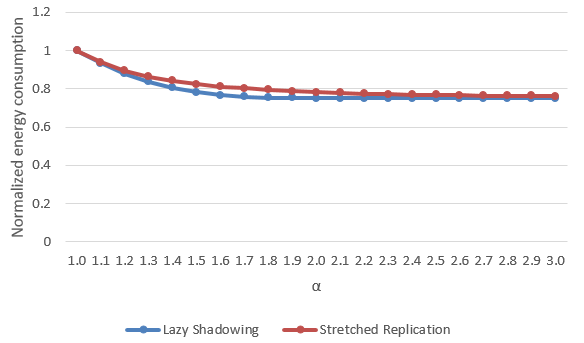
\includegraphics[width=\columnwidth]{figures/alpha_1.png}
		}
		\subfigure[$\rho=0.3$]
		{
			\label{fig:alpha_2}
			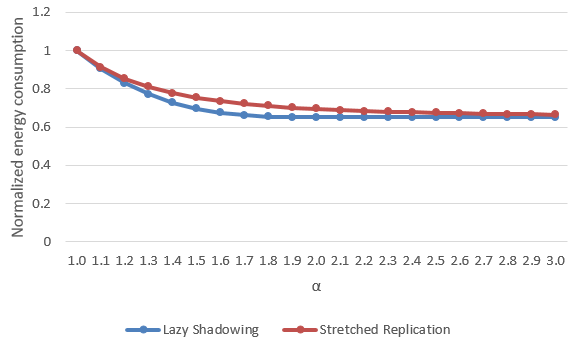
\includegraphics[width=\columnwidth]{figures/alpha_2.png}
		}
	\end{center}
	\caption{Normalized energy consumption for various response time laxities. W=240 hours, MTBF=5 years.}
	\label{fig:alpha}
\end{figure}


Figure~\ref{fig:alpha} shows that both lazy shadowing and stretched replication can achive over 20\% of energy savings compared to state machine repilcation, when there is enough laxity in the response time. When there is no laxity in the response time ($\alpha=1$), lazy shadowing and stretched replication don't have any freedom to reduce the execution rate of the shadow process, thus will execute both the main and shadow processes at the maximal execution rate, which essentially converges to state machine replication. In this case, it is staightforward that all three approaches have the same energy consumption. However, as laxity in response time increases, lazy shadowing and stretched replication immediately gain the ability to slow down the shadow process and thus save energy. It is also clear that laxy shadowing has more potential than stretched replication in energy saving. It can take better advantage of the laxity in respone time as it is more flexible in controling the execution rate than stretched replication. The highest difference is 4.5\% when $\alpha$ is around 1.5. As the laxity keeps increasing, the energy savings by lazy shadowing and stretched replication flatten out, as a result of the static power consumption. Since the static power consumption is independent of the execution rate, reducing the execution rate would extend the execution time, resulting in an increase in the energy consumption corresponding to the static power. Therefore, the minimal energy consumption would be achieved when there is a balance between energy from dynamic power and energy from static power, which may not be necessarily equivalent to using all the laxity in response time. It can be projected that if the staic power ratio is lower, laxy shadowing and stretched replication can take advantage of more laxity and achieve more energy saving compared to state machine replication. This will be discussed further in later section. At the right side of Figure~\ref{fig:alpha_1} and Figure~\ref{fig:alpha_2}, lazy shadowing and stretched replication converge when there is enough laxity for both of them. 

\subsection{Task vulnerability}
The objective of lazy shadowing is to minimize the expected energy consumption, considering the characteristics of both the task to execute and the underlying system. The probability of failure during the execution of the task is an important factor that will impact how the proposed fault tolerance approaches execute the task. Specifically, they will choose different process execution rates according to the likelyhood of failures. The ratio between the task workload and the MTBF is an approximation of the likelyhood of failure, assuming task workload is far less than the MTBF. In our experiments, we find that there is a linear relationship between task workload and MTBF in determining the optimal execution rates. Specifically, increasing the task workload has the same effect as decreasing the MTBF in our analytical models. Therefore, we combine them as a single parameter and refer to it as task vulnerability.

\begin{figure}[!t]	
	\begin{center}
		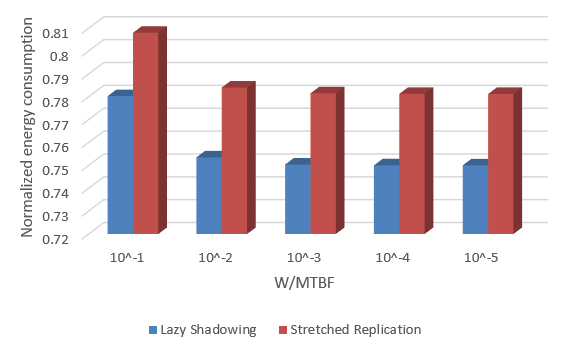
\includegraphics[width=\columnwidth]{figures/vulnerability.png}
	\end{center}
	\caption{Normalized energy consumption for various task vulnerabilities. $\rho$=0.5.}
	\label{fig:vulnerability}
\end{figure}

The results of the sensitivity study to task vulnerability, when $\rho=0.5$, are shown in Figure~\ref{fig:vulnerability}. From left to right, the task vulnerability decreases, meaning that the likelyhood of failure decreases. We can see that for all task vulnerabilities considered, both lazy shadowing and stretched replication can achieve significant energy savings over state machine replication. This indicates that the proposed approaches are scalable to future large-scale and failure-prone HPC environments. As task vulnerability decreases, lazy shadowing and stretched replication gains more energy savings. This is because the probability that the main process can complete the task without failure increases when task vulnerability decreases, increasing the probability that the shadow process can be terminated early to save energy. Again, lazy shadowing outperforms stretched replication because of its more flexibility in controling the execution rate of its shadow process.

\subsection{Static power ratio}
The computing nodes of each supercomputers have different power consumption characteristics, depending on the various computer organization and architecture technologies. Since our approaches are based on DVFS to control the process execution rates, the power consumption is partitioned into dynamic power, which has a superlinear relationship with the execution rate, and static power, which is unaffected by the execution rate. Static power ratio is an effecitve way to abstract the power saving ability of the proposed approaches on different machines.

\begin{figure}[!t]	
	\begin{center}
		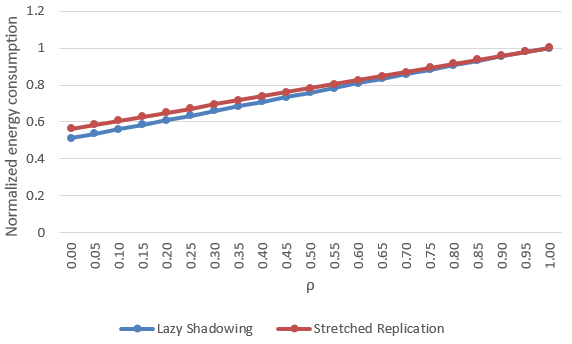
\includegraphics[width=\columnwidth]{figures/rho.png}
	\end{center}
	\caption{Normalized energy consumption for various static power ratios. W=240 hours, $\alpha$=2, MTBF=5 years.}
	\label{fig:rho}
\end{figure}

DVFS saves dynamic power while not changing static power. These two aspects have conflicting effects on the total energy consumption. By reducing the execution rate, the execution time increases proportionally. This also increases the energy consumption from static power proportionally as the static power is constant. However, since the dynamic power can be reduced superlinearly, the energy consumption corresponding to dynamic power is reduced, even though the execution is extended. The above analysis can be illustrated with Figure~\ref{fig:rho}. In addition, Figure~\ref{fig:rho} reveals that lazy shadowing can save up to 49\% of energy over state machine replication when consider dynamic power only. On the other hand, lazy shadowing and stretched replication are forced to execute both the main and shadow processes at the maximal rate when dynamic power is negligible, converging to the behavior of state machine replication. Current supercomputers have a static power ratio between 40\%-70\%, and it is reasonable to suspect that this will continue to be the case. Within this range, the energy saving is 14\%-29\% for lazy shadowing, and 13\%-26\% for stretched replication.



\section{Conclusion}
\label{conclusion}
%Current fault-tolerance approaches rely exclusively on either time or hardware redundancy for recovery. Rollback recovery  exploits time redundancy but can incur significant delay and high energy cost. On the other hand, process replication relies on hardware redundancy and requires a significant increase in resources and  power consumption.

In this paper, we propose Rejuvenating Shadows as a novel power-aware fault tolerance model, which guarantees forward progress, maintains consistent level of resilience, and minimizes implementation complexity and runtime overhead. Empirical experiments demonstrated that the Rejuvenating Shadows model outperforms in-memory checkpointing/restart in both execution time and resource utilization, especially in failure-prone environments.

Leaping induced by failure has proven to be critical in reducing the divergence between a main and its shadow, 
%with respect to workload execution.
%Consequently, the time to recover from subsequent failures is reduced significantly. 
thus reducing the recovery time for subsequent failures. Consequently, the time to recover from a failure increases with failure intervals.  
Based on this observation, a proactive approach is to ``force" leaping when the divergence between a main and its shadow exceeds a specified threshold. 
In our future work, we will further study this approach to determine what behavior triggers forced leaping in order to optimize the average recovery time. 

%we will study forcing the shadDuring experimentation we noticed the problem that recovery time in Rejuvenating Shadows can become substantial when the failure interval is large (Figure~\ref{fig:single_failure}). To deal with this issue, we are studying the idea of ``forced leaping", which borrows the idea from periodic checkpointing and forces a leaping whenever failure has been absent for a long time, in order to reduce the divergence between mains and shadows. Optimal intervals for forced leaping will be explored to balance between runtime overhead and failure recovery overhead. 

%In the future we plan to explore the integration with fault prediction techniques and the viability of dynamic and partial shadowing for platforms where nodes exhibit different ``health" status, e.g., some nodes may be more reliable while others are more likely to fail~\cite{gainaru2012fault}. 
%With this taken into account, we can apply dynamic scheduling of shadows only for mains that are likely to fail, to further reduce the resource requirement. 
%Another future direction is to study complier-assisted program slicing for fault detection. Specifically, slices that are fraction of their mains can run lazily as shadows and provide fault detection capability with reasonable coverage. 





\bibliographystyle{abbrv}
%\bibliographystyle{ieee}
\bibliography{icpp2013}

\end{document}
